\mynewpage
\chapter{Rotations}

\section{To Do}

\begin{itemize}
\item Include my lect notes on exp and log and rodrigues from soatto -- GOOD
\item cite this: Metrics for 3D Rotations: Comparison and Analysis JMIV 2009
\end{itemize}


\section{Usual representations of rotation}
We have three majorly used representations: Matrices,
Axis-angle, and Quaternions, as reviewed below.

\section{Matrices}
In terms of roll, pitch, and yaw angles, as in Figure~\ref{fig:yaw:pitch:roll}, the rotation matrix $R = \mathcal M^A_B(id)$ can be decomposed
as $R(\theta,\phi,\psi) =
R_z(\theta)R_y(\phi)R_x(\psi)$, where
\begin{align}
R_z(\theta) &= \begin{bmatrix}
\cos\theta & \sin\theta & 0\\
-\sin\theta & \cos\theta & 0\\
0 & 0 & 1
\end{bmatrix}\\
%
R_y(\phi) &= \begin{bmatrix}
\cos\phi & 0 & -\sin\phi\\
0 & 1 & 0\\
\sin\phi &0 &\cos\phi
\end{bmatrix}\\
%
R_x(\psi) &= \begin{bmatrix}
1 & 0 & 0\\
0 & \cos\psi & \sin\psi\\
0 &-\sin\psi & \cos\psi
\end{bmatrix}
\end{align}

And the form of $R(\theta,\phi,\psi) = R_z(\theta)R_y(\phi)R_x(\psi)$ would be:
\begin{align}
\begin{bmatrix}
\cos\theta\cos\phi & \cos\theta\sin\phi\sin\psi + \sin\theta\cos\psi & 
-\cos\theta\sin\phi\cos\psi + \sin\theta\sin\psi\\
%
-\sin\theta\cos\phi & -\sin\theta\sin\phi\sin\psi + \cos\theta\cos\psi &
\sin\theta\sin\phi\cos\psi + \cos\theta\sin\psi\\
%
\sin\phi & -\cos\phi\sin\psi & \cos\phi\cos\psi
\end{bmatrix}
\end{align}
Note that this is the inverse of the rotation for points while fixing the bases. 
Note also that the order of multiplication of the $x,y,z$ rotation matrices
makes a difference in the final rotation.
\begin{figure}
\centering
   \subfigure[]{ %
    \label{fig:yaw:pitch:roll}
      \begin{minipage}[c]{0.45\linewidth}%
         \centering
        \scalebox{0.4}{\includegraphics{figs/yaw-pitch-roll.eps}}
      \end{minipage}}
    \subfigure[]{ %
      \label{fig:axis:angle}
      \begin{minipage}[c]{0.45\linewidth}%
         \centering
         \scalebox{0.4}{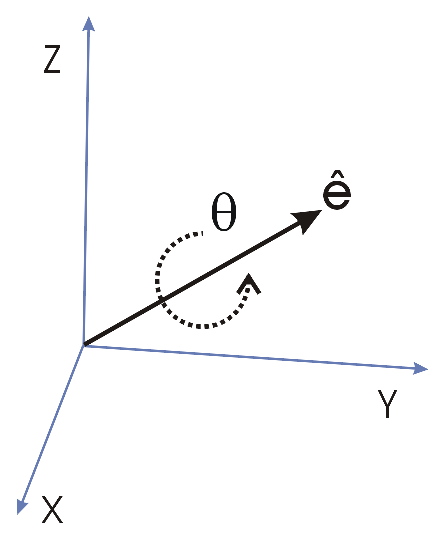
\includegraphics{figs/Euler_AxisAngle.eps}}
      \end{minipage}}
\caption{% 
(a) Orthogonal rotations; (b)
Any 3D rotation can be represented by a rotation of angle $\theta$ around an
axis $\hat{\mathbf{e}}$
}
\end{figure}

\paragraph{Normalization}
When rotation matrices are computed from measured points and camera
observations, it is typical that the resulting rotation matrix does not
satisfy the orthonormal constraints that must hold among the rows and columns.
In order to normalize a 3x3 matrix to insure that it is orthonormal the following operation must be performed:
\begin{equation}\label{eq:r:normalized}
R_{normalized} = R\left[ \left( R^\top R \right)^{\frac{1}{2}}
\right]^{-1}
\end{equation}


\paragraph{Pros}
\begin{itemize}
\item Fastest for rotating large ammounts
of point data, according to~\cite{Schneider:Geometry:book:2003}.
\end{itemize}
\paragraph{Cons}
\begin{itemize}
\item Slower than quaternion for composing rotations
\item Slower than quaternion for normalization that is used due to round-off errors that
occur during optimization. 
\item Problems due to singularities
\item Has 9 parameters (all entries of the $3\times 3$ matrix), even though rotations have 3 degrees of freedom
\end{itemize}

\section{Quaternions}

\todo{I have an improved version with Soatto' insights on $\mathbb C + \mathbb C j$}

The quaternion is a 4-D vector analogous to the complex number. Rotations can be represented as unit
quaternions. In order to define product of quaternions, its 4 parameters
are grouped into a 3D vector part and a scalar part along with an associated algebra:
\begin{align}
q &= q_0 + \mathbf q = q_0 + iq_1 + jq_2 + kq_3
\intertext{Where $i,j,k$, the hypercomplex numbers, play a similar role to the imaginary axis in complex
numbers. The conjugate of a quaternion is defined as:}
q^* &= q_0 - \mathbf q
\shortintertext{Its magnitude is:}
|q| &= qq^* = (q_0 + \mathbf q)(q_0 - \mathbf q) = q_0^2 - \mathbf q\mathbf q
\end{align}
The meaning of $\mathbf q\mathbf q$ comes from the axioms for multiplying the
$i,j,k$ components:
\begin{align}
i^2 &= j^2 = k^2 = -1\\
ij &= k,\,\, ji = -k\\
jk &= i,\,\, kj = -i\\
ki &= j,\,\, ik = -j
\end{align}
In order to multiply quaternions, just use usual distributive laws, being careful
with the order, and applying the above axioms. The meaning of multiplication is
more clear if we first consider the product of two different quaternion vectors:
\begin{align}
&\mathbf p\mathbf q = (ip_1 + jp_2 + kp_3)(iq_1 + jq_2 + kq_3) =\notag\\
&i(p_2q_3 - p_3q_2) + j(p_3q_1 - p_2 q_3) + k(p_1q_2 - p_2q_1) - (p_1q_1 + p_2q_2
+ p_3q_3) = \notag\\
&\mathbf p\times\mathbf q - \mathbf p\cdot \mathbf q
\end{align}
It follows that 
\begin{align}
\mathbf q\mathbf q &= \mathbf q\times\mathbf q - \mathbf q\cdot\mathbf q =
-(q_1^2 + q_2^2 + q_3^2)
\shortintertext{so:}
qq^* &= (q_0^2 + q_1^2 + q_2^2 + q_3^2) = |q|^2
\end{align}
which is a reasonable interpretation of a conjugate operation.
The inverse of a quaternion is:
\begin{equation}
\mathbf q^{-1} = \frac{q^*}{|q|^2}
\end{equation}
The rotation about a unit vector $\hat{\mathbf e}$ is:
\begin{equation}
q = \cos \frac{\theta}{2} + \sin \frac{\theta}{2}\hat {\mathbf e}
\end{equation}
Note that $|q| = 1$. We can encode a regular 3-vector $\Gama$ as a
quaternion as $\Gamma = 0 + \Gama$. The rotation of this vector is defined as:
\begin{equation}
\Gamma' = q\Gamma q^*
\end{equation}

\paragraph{Example.} 
To illustrate consider a point in the $x-y$ plane which is on the $x$ axis,
$\Gama = (2,0,0)$. Rotate the point around the z axis by 90 degrees. The
rotation is expressed as:
\begin{equation}
q = \cos 45^\circ + \sin 45^\circ (0i + 0j + k) = 0.707 + 0.707k
\end{equation}
The rotation of $\Gama$ is:
\begin{equation}
\Gamma' = (0.707 + 0.707k)(0 + 2i)(0.707 - 0.707k) = 0 + 0i + j + 0k
\end{equation}
which is a vector along the $y$ axis, as expected.

Composing two rotations $p$ and $q$ is just the product, so that:
\begin{equation}
\Gamma' = (pq)\Gamma(pq)^*
\end{equation}

\paragraph{Quaternion to Rotation Matrix}
\begin{equation}\label{eq:quaternion:to:rotation:matrix}
q\Gamma q^* \rightarrow
\begin{bmatrix}
q_0^2 + q_1^2 - q_2^2 - q_3^2 & 2(q_1q_2 - q_0q_3) & 2(q_1q_3 + q_0q_2)\\
2(q_1q_2+q_0q_3) & q_0^2 - q_1^2 + q_2^2 - q_3^2 & 2(q_2q_3 - q_0q_1)\\
2(q_1q_3 - q_0q_2) & 2(q_2q_3 + q_0q_1) & q_0^2 - q_1^2 -q_2^2 + q_3^2
\end{bmatrix}
\Gama,
\end{equation}
with $q_0^2 + q_1^2 + q_2^2 + q_3^2 = 1$.

\paragraph{Rotation Matrix to Quaternion}
\begin{equation}
R = 
\begin{bmatrix}
r_{00} & r_{01} & r_{02}\\
r_{10} & r_{11} & r_{12}\\
r_{20} & r_{21} & r_{22}
\end{bmatrix}
\end{equation}
\begin{equation}
q_0 = \frac{1}{2}\sqrt{r_{00}^2 + r_{11}^2 + r_{22}^2},\,\,
q_1 = \frac{r_{21} - r_{12}}{4q_0},\,\,
q_2 = \frac{r_{02} - r_{20}}{4q_0},\,\,
q_3 = \frac{r_{10} - r_{01}}{4q_0}
\end{equation}

\paragraph{Axis-angle to Quaternion}
As noted above, the rotation about a unit vector $\hat{\mathbf e}$ is:
\begin{equation}
q = \cos \frac{\theta}{2} + \sin \frac{\theta}{2}\hat {\mathbf e}
\end{equation}
Note that $|q| = 1$. 

\paragraph{Normalization}
In order to normalize a quaternion to be unit, we simply do:
\begin{equation}
q_{normalized} = \frac{qq^*}{|q|^2}
\end{equation}
Compared to~\eqref{eq:r:normalized}, this is a lot cheaper.


\paragraph{Pros}
\begin{itemize}
\item Said do be the best for optimization. Vxl uses it, Faugeras uses it.
\draftnote{TODO: clarify}
\item Useful to give solvable algebraic equations involving rotations, by
using~\ref{eq:quaternion:to:rotation:matrix}.  Astr\"om~\cite{Astrom:etal:Polysolver:IJCV09} uses it. 
\item Easy to compose through multiplication. Faster than matrices for this.
\item Normalization is very fast compared to matrices
\item No singularity in the parametrization
\end{itemize}

\paragraph{Cons}
\begin{itemize}
\item Slower than rotation matrices for transforming points. However, difference
is negligible for large number of points.
\draftnote{todo: quantify}
\item 4 parameters for the 3 degrees of freedom of rotation matrices
\end{itemize}

\paragraph{Research directions}
Study quaternions in:
\begin{itemize}
\item Penrose's ``The Road to Reality'' book has a good chapter on quaternions,
clifford and grassman algebras.
\item Wikipedia about quarternions and rotations.
\item Book on rotations, quaternions and double groups
\item (Vague): Recall that Stolfi's oriented projective geometry has more to do with
rotation geometry.
\end{itemize}

\section{Axis-Angle}

We can represent any 3D rotation by a rotation around a rotation axis
$\hat{\mathbf e}$ and angle $\theta$. This can be encoded as $\mathbf e =
\theta\cdot\hat{\mathbf e}$, i.e.\ a vector whose direction is the axis of
rotation, and the magintude is the angle of rotation around such axis.

\paragraph{Axis-Angle to Rotation Matrices}

To convert from the axis-angle to a rotation matrix, we use the Rodrigues
formula~\cite{Ma:Soatto:etal:book}:

\begin{equation}\label{eq:rodrigues:rotation:formula}
R(\theta,\hat{\mathbf e}) = I + \frac{\sin\theta}{\theta} \hat{\mathbf e}_\times
+ \frac{(1 - \cos\theta)}{\theta^2}\hat{\mathbf e}_\times^2
\end{equation}
where
\begin{align}
\hat{\mathbf e} &= 
\left[ a\,\,b\,\,c \right]^\top\\
\hat{\mathbf e}_\times&= \left[\begin{array}{ccc} 0 & -c & b\\ c & 0 & -a\\ -b &
a & 0 \end{array} \right]
\end{align}

\paragraph{Rotation Matrices to Axis-Angle.}
Eigen-decomposition of the rotation matrix yields the eigenvalues $1$, and $\cos\theta \pm i\sin\theta$.
The Euler axis is the eigenvector corresponding to the eigenvalue of $1$, and the $\theta$ can be computed from the remaining eigenvalues.


\paragraph{Pros}
\begin{itemize}
\item Due to the Rodrigues formula, it seems easy to use this representation in
equations
\end{itemize}

\paragraph{Cons}
\begin{itemize}
\item Hard to compose two transformations
\item Prone to singularities
\end{itemize}

\section{Exponential maps}

TODO: merge in notes from Taubin, Ma's book, and other sources.

\section{Cayley Rational Parametrization}
TODO: merge in notes from Taubin

\section{Estimating Rotations}
Rotations and rigid motions in general can be estimated from noisy 3D-3D point
correspondences using procrustes analysis (see e.g.\ Matlab's procrustes
function in the statistics toolbox). Minimal problems involving rotation seem hard to
solve. These problems can be found in inverse kinematics in robotics books. See
Horn's robotics book or Paul's book from MIT press, or even a chapter
in~\cite{Cox:etal:Ideals}. The state-of-the-art techniques for robustly estimating models
that involve rotation is, to the best of our knowledge, Kalle Astr\"om's
work~\cite{Astrom:etal:Polysolver:IJCV09} on minimal solvers together with
RANSAC.  

Here is a practical way of estimating a rotation matrix in Matlab, given 4
known vectors transformed to other 4 known vectors:
\begin{verbatim}
%
% Generate a random rotation matrix
%
[Q dummy]= qr(rand(3));
Q

%
% Random 4 vectors in R^3 in the first coordinate
%
A=randn(3,4);
B=Q*A; % Coordinates in the second system

%
% Estimates Q from A and B
%
Qest = B/A

%
% Do this if you don't trust your data and
% want to reorrthogonalize Qest
%
[U,S,V]=svd(Qest);
Qest = U*V'
\end{verbatim}

Here is a way of estimating using procrustes:
\begin{verbatim}
 >> A = randn(4,3); % four random vectors in 3-D
 >> [U,S,V] = svd(randn(3)); T = U*V'; % random orthogonal matrix
 >> T
T =
      -0.91586 -0.14665 -0.37375
      0.084785 0.83926 -0.53707
       0.39244 -0.52357 -0.75621
 >> B = A*T; % rotate A
 >>
 >> [d,B1,tr] = procrustes(B,A);
 >> tr.T % rotation component: same as original T
ans =
      -0.91586 -0.14665 -0.37375
      0.084785 0.83926 -0.53707
       0.39244 -0.52357 -0.75621
 >> tr.c % translation component: 0
ans =
    2.2204e-16 5.5511e-17 0
    2.2204e-16 5.5511e-17 0
    2.2204e-16 5.5511e-17 0
    2.2204e-16 5.5511e-17 0
 >> tr.b % scale component: 1
ans =
             1
\end{verbatim}

Question: is 4 vectors the minimum needed to get $\rot$?

\subsection{Rotation minimizing turning angle}

Given unit vectors $\vec v$ and $\vec w$, we can use Rodrigues'
formula~\eqref{eq:rodrigues:rotation:formula} to compute the rotation that
minimizes the turning angle amongst all the rotations that take $\vec v$ to
$\vec w$. We just write
\begin{equation}
\rot(\theta,\hat{\mathbf e}) = I + \sqrt{1 - (\vec v^\top\vec w)^2}\hat{\mathbf e}_\times
+ \vec v^\top\vec w\hat{\mathbf e}_\times^2,
\end{equation}
with $\hat \e = \frac{\vec v \times \vec w}{\sqrt{1 - (\vec v^\top\vec w)^2}}$.
If $\vec v =  \vec w$, we simply define the minimal rotation to be the identity
matrix. If $\vec v =  -\vec w$ we have a singularity in the
$\rot(\theta,\hat{\mathbf e})$ function.
